\chapter{Kielimallien vertailu}%
\label{ch:vertailu}

\begin{itemize}
  \item Kuinka tärkeitä mitkäkin ominaisuudet, mitä painotetaan yms.
  \item Mitkä ovat kriteerit
  \begin{itemize}
    \item Onko jo käytettävissä (vapaasti käytettävissä vai vasta jotain kevyitä trialeita, joilla ei voi oikeasti tehdä mitään)?
    \item Onko käytettävissä millaisella työmäärällä?
    \item SaaS vs itse-hostattava tms.?
    \item Hinta
    \item Miten hyvin suoritutuu annetusta tehtävästä?
    \item Miten hyvin käsittelee "huonoja tilanteita" (esim. syöte on onnetonta, tuottaako mitään järkevää tai saako tiedon ettei syöte ollut hyvää tms.)
    \item Toimiiko suomeksi vai tarvitaanko erillinen kääntäminen?
  \end{itemize}
  \item Joku vertailutaulukko?
  \item  Käytännössä kaikki seuraavista on transformer arkkitehtuurin päälle rakennettuja etukäteen koulutettuja.
  \begin{itemize}
    \item GPT
    \begin{itemize}
      \item Generative pre-trained transformer
      \item OpenAI:n kehittämä
    \end{itemize}
    \item BERT
    \begin{itemize}
      \item Bidirectional Encoder Representations from Transformers
      \item Googlen kehittämä
      \item Encoder only (https://huggingface.co/learn/nlp-course/chapter1/5)
    \end{itemize}
    \item LLaMA
    \begin{itemize}
      \item Large Language Model Meta AI
      \item Metan kehittämä
      \item https://ai.meta.com/llama/
    \end{itemize}
    \item Bloom
    \begin{itemize}
      \item BigScience Large Open-science Open-access Multilingual Language Model
      \item Useamman tahon kehittämä
      \item Modified from Megatron-LM GPT2
      \item Decored only
    \end{itemize}
    \item FinBERT
    \item Finnish GPT-3
  \end{itemize}
  \item https://huggingface.co/AaltoSpeech
  \begin{itemize}
    \item CombFinnish-AED-CRDNN / Automatic Speech Recognition / Jonkin sortin puheentunnistusta?
  \end{itemize}
  \item https://huggingface.co/Helsinki-NLP
  \begin{itemize}
    \item simple-finnish-gpt3-xl / Text Generation / finetuned versio TurkuNLP/gpt3-finnish-xl:sta
  \end{itemize}
  \item https://huggingface.co/TurkuNLP
  \begin{itemize}
    \item bert-base-finnish-cased-v1, vertailujen mukaan parempi kuin Googlen multilingual (https://github.com/google-research/bert/blob/master/multilingual.md)
    \item löytyy myös uncased versio
    \item löytyy large variant
    \item toxicity versio, joka ilmeisesti tunnistaa 6 eri tyyppistä toxicityä
    \item QA versio
    \item bloom-finnish-176b / Text Generation / rakennettu bloom:in päälle sisältämään suomenkielisiä datasettejä
    \item gpt3-finnish-X / Text Generation / useampi erikokoinen GPT-3-malli, "puhtaita kielimalleja" eli ei ole hienosäädetty mm. vuoropuheluun tai kysymyksiin
    \item sbert-cased-finnish-paraphrase / Sentence Similarity / tunnistaa virkkeiden samankaltaisuutta
  \end{itemize}
  \item https://huggingface.co/Finnish-NLP
  \item https://huggingface.co/Kansallisarkisto
  \begin{itemize}
    \item finbert-ner / Token Classification / tunnistaa nimiä yms. tekstistä, hienosäädetty versio TurkuNLP/bert-base-finnish-cased-v1:sta
  \end{itemize}
  \item https://huggingface.co/tasks
  \item https://huggingface.co/models?pipeline\_tag=text-generation\&language=fi\&sort=trending
  \item https://huggingface.co/Finnish-NLP/llama-7b-finnish
  \item https://huggingface.co/TurkuNLP/gpt3-finnish-3B
\end{itemize}

\section{Google Gemini}

Gemini on Googlen julkaisema kielimalliperhe, jonka on seuraaja PaLM 2:lle
\parencite{googleKeynote2023}. Googlella on myös Gemini-niminen ChatBot, joka
tunnettiin aiemmin nimellä Bard, ennen kuin Google nimesi sen uudelleen
Geminiksi \parencite{geminiUpdates}. Geministä on useita eri malleja, jotka on
tarkoitettu eri käyttötilanteisiin. Näitä malleja ovat Ultra, Pro, Flash ja
Nano. \parencite{googleDeepmindGemini} Näistä Ultra on tarkoitettu
monimutkaisimpiin tehtäviin, Pro optimoitu kustannusten ja viiveen kannalta ja
Nano puolestaan laitteissa pyöritettäväksi
\parencite{googleDeepmindGeminiv1report}. Flash puolestaan on entistä
kustannustehokkaampi ja nopeampi kuin Pro \parencite{googleKeynote2024}.
Malleista on useita eri versioita, jotka on välillä nimetty samoin kuin
edelliset versiot \parencite{googleDeepmindGeminiv1_5report}. Kehitys on ollut
erittäin nopeaa ja versiot vanhenevat nopeasti uusien tullessa käytettäviksi.

% TODO: lyhyesti teoriaa, mihin kielimallit pohjautuvat?

Gemini ei ole saatavilla Googlen AI Studion kautta ilman maksullista tilausta
Suomessa \parencite{googleAiAvailableRegions}. Geminiä on kuitenkin mahdollista
käyttää Vertex AI -alustan kautta.

Gemini 1.0 Pron hinta syötteenä annetuille kuville on \$0.0025 / kuva, videolle
\$0.002 / sekunti, tekstille \$0.000125 / 1000 merkkiä ja ulostulolle
\$0.000375 / 1000 merkkiä. Gemini 1.5 Pron hinnat ovat noin puolet syötteelle
eli kuville \$0.001315 / kuva, videoille \$0.001315 / sekunti, tekstille
\$0.00125 / 1000 merkkiä ja äänelle \$0.000125 / sekunti. Ulostulo puolestaan
on 10-kertaa kalliimpi eli \$0.00375 / 1000 merkkiä. Gemini 1.5 Pron hinnat
kaksinkertaistuvat mikäli käytössä oleva konteksti on yli 128 000. Gemini
1.5 Flashin hinnat ovat 10\% siitä mitä Gemini 1.5 Pron hinnat ovat.
\parencite{vertexAiGenerativeAiPricing} Hintoja on havainnollistettu taulukossa
\ref{tab:vertex-ai-generative-ai-pricing}.

\begin{table}[H]
  \centering
  \rowcolors{2}{gray!25}{white}
  \caption{Esimerkki hintoja eri syötteille ja ulostuloille}
  \label{tab:vertex-ai-generative-ai-pricing}
  \begin{tabular}{lccc}
    \textbf{Esimerkki} & \textbf{Gemini 1.0 Pro} & \textbf{Gemini 1.5 Pro} & \textbf{Gemini 1.5 Flash} \\
    \hline
    \Gape[0pt][2pt]{\makecell[l]{Syöte: 500 merkkiä\\Ulostulo: 1000 merkkiä}} & 0,041 snt & 0,408 snt & 0,041 snt \\
    \Gape[0pt][2pt]{\makecell[l]{Syöte: 1 kuva\\Ulostulo: 1000 merkkiä}} & 0,27 snt & 0,47 snt & 0,047 snt \\
    \Gape[0pt][2pt]{\makecell[l]{Syöte: 10 minuutin video\\Ulostulo: 1000 merkkiä}} & 1,123 € & 0,739 € & 0,074 € \\
    \Gape[0pt][2pt]{\makecell[l]{Syöte: 30 minuuttia ääntä\\Ulostulo: 1000 merkkiä}} & - & 0.213 € & 0.021 € \\
    \hline
  \end{tabular}
\end{table}

\section{PaLM 2}

PaLM:n uudempi versio, PaLM 2, on Googlen 2023 loppukeväällä julkaisema
kielimalli. Kielimallista tehtiin useampi erikokoinen malli: Gecko, Otter,
Bison ja Unicorn. Näistä pienin, Gecko, oli mitoitettu toimimaan puhelimissa ja
mahdollistamaan kielimallin käyttäminen ilman internet-yhteyttä. Näiden lisäksi
toteutettiin muun muassa lääketieteellisellä datalla hienosäädetty Med-PaLM 2.
\parencite{googleKeynote2023} \parencite{googlePaLM2Introducing}

PaLM 2:n kouluttamiseen käytettiin muun muassa verkkodokumentteja, kirjoija,
koodia, matematiikkaa ja keskusluita. PaLM 2:n koulutuksessa huomioitiin
merkittävästi paremmin useat eri kielet. \parencite{googlePaLM2TechReport}

Sittemmin muun muassa PaLM API on deprekoitu ja kehittäjiä on suositeltu
siirtymään Geminin pariin \parencite{googlePaLMAPIDeprecated}. Myös hinnoittelu
ja maininta Bison Text ja Chat -malleista on poistettu, vaikka malleja on vielä
mahdollista käyttää 2024 alkukesästä Vertex AI:n kirjastojen avulla.

\section{Claude}

Tekoälyn turvallisuuteen ja tutkimukseen keskittyvä yritys, Anthropic, on
luonut oman tekoälynsä, Clauden. Claude on pyritty rakentamaan
tietoturvalliseksi, luotettavaksi ja varmaksi. \parencite{anthropicCompany}
\parencite{anthropicClaude} Näihin on pyritty esimerkiksi tutkimuksien avulla,
jotka ovat keskittyneet muun muassa suojauksen murtamisen (jailbreaking)
estämiseen. \parencite{anthropicResearch}

Nykyisin Claudesta on kolme eri mallia versiolla 3.0. Näitä malleja ovat
Sonnet, Opus ja Haiku. Pääasiallisesti Opus on isoin ja paras malli kun Haiku
puolestaan keskittyy nopeuteen ja on huomattavasti pienempi. Sonnet puolestaan
jää näiden kahden välimaastoon. Sonnetista on kuitenkin julkaistu uudempi
versio 3.5, joka on saatu Opus:ta paremmaksi kuitenkin pitäen kulut samana kuin
3.0 versiossa. Tilannetta on havainnollistettu kuvassa
\ref{fig:3-5-sonnet-curve}. \parencite{anthropicAPIDocsModels}

\begin{figure}[H]
  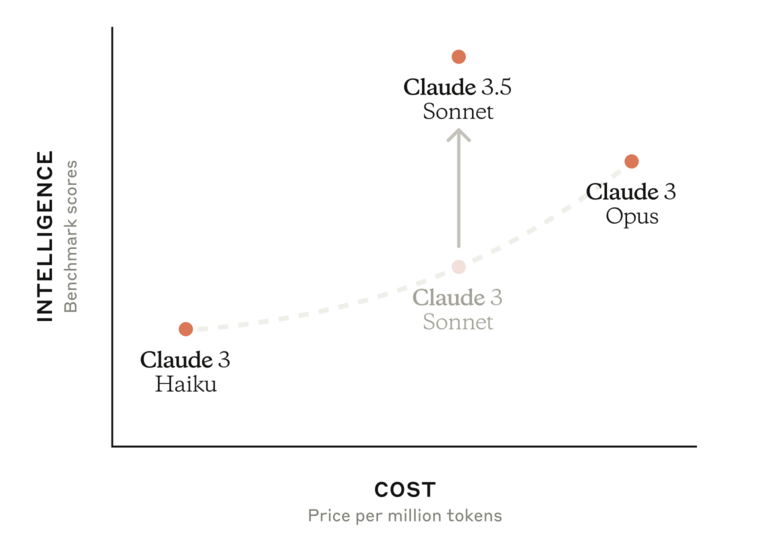
\includegraphics[width=\textwidth]{figures/3-5-sonnet-curve.png}
  \caption{Anthropic API dokumentaatiossa oleva havannollistava kuva mallien eroista 05.08.2024}
  \label{fig:3-5-sonnet-curve}
\end{figure}

Claudea on mahdollista kokeilla web-käyttöliittymän kautta rekisteröitymisen
jälkeen ilmaisena muutamia kyselyitä päivässä \parencite{claudeChat}. Tarjolla
on myös Anthropic API, joka vaatii aktiivisen tilauksen. APIa voi käyttää
tarjolla olevien kirjastojen avulla tai vaihtoehtoisesti suorittaa itse kutsuja
API-dokumentaation mukaisesti. Claude on saatavilla myös AWS Bedrockin sekä
Vertex AI:n kautta. \parencite{anthropicAPIDocs}

Clauden hinnoittelu vaihtelee hiukan sivuston mukaan. Claude.ai:n Pro-tilauksen
hinnoiksi ilmoitetaan \$20 tai 18€ + ALV ja Team-tilaukselle \$25/\$30 tai
23€/28€ + ALV. \parencite{anthropicPricing} \parencite{claudePricing} Anthropic
API:n hinnat on esitetty taulukossa \ref{tab:anthropic-api-pricing}

\begin{table}[H]
  \centering
  \rowcolors{2}{gray!25}{white}
  \caption{Anthropic APIn hinnat}
  \label{tab:anthropic-api-pricing}
  \begin{tabular}{lccc}
    \textbf{Malli} & \textbf{Syöttö} & \textbf{Ulostulo} \\
    \hline
    Claude 3.5 Sonnect &    \$3 / MTok &   \$15 / MTok \\
    Claude 3 Opus      &   \$15 / MTok &   \$75 / MTok \\
    Claude 3 Haiku     & \$0.25 / MTok & \$1.25 / MTok \\
    \hline
  \end{tabular}
\end{table}

Clauden ilmainen tilaus sisältää vain Claude 3.5 Sonnetin käyttämisen web-
käyttöliittymän sekä sovellusten kautta. Pro-tilaus lisää mahdollisuuden
käyttää Opus- ja Haiku-malleja sekä joitain QoL-lisäyksiä ja suurempaa
prioriteettia käyttäjälle. Team-tilaus on lähinnä tiimin hallinnan ja maksun
kannalta oleellisia lisätoiminnallisuuksia. Pro-tilaus lisää viisin kertaisen
käyttörajan verrattuna ilmaiseen ja Team-tilaus sitäkin suuremman.
\parencite{anthropicPricing} \parencite{claudePricing} Selviä käyttörajoja ei
ole saatavilla.
